% A sample model to write a TFG project

% IMPORTANT!!! Substitute "draft" with "final" to render the final version of the TFG 
\documentclass[titlepage,openright,twoside,a4paper,draft,12pt,spanish]{book}

% Configuring the environment to support spanish characters.
\usepackage[T1]{fontenc}
\usepackage[utf8]{inputenc}
\usepackage[spanish]{babel}
\selectlanguage{spanish}

\usepackage[pdftex,final]{graphicx}

% Style package
\usepackage{trinidad-TfG}
% Font Package (Palatino)
\usepackage{mathpazo}
% Packages for specific capabilities
\usepackage{rotating} % for text rotation in tables
\usepackage{multirow} % for multirow in tables
\usepackage{subfigure} % Place subfigures in figure environment
% Packages for specific symbols
\usepackage{amssymb}
\usepackage{amsmath}
\usepackage{amsfonts}
\usepackage{eurosym} % Euro symbol
\usepackage{bbding} % for \XSolidBrush
\usepackage{pifont} % for \ding{55} (a check mark)

\author{Nombre del Alumno}{Grado en Ingeniería Informática - Especialidad}{D.~}{12345678A}
\authorURL{http://www.lsi.us.es/~trinidad}
\authorEMail{ptrinidad@us.es}
\setTitle{Título del Trabajo Fin de grado}
%\setSubtitle{No subtitle}
\setUniversity{Universidad de Sevilla}
\copyrightText{Pon aquí cuestiones acerca del copyright}
\supervisor{Pablo Trinidad Martín-Arroyo}{Dr.~}{Lenguajes y Sistemas Informáticos}



\makeglossaries
\begin{document}
\makeTitlePage

\pagestyle{empty}
\begin{dedication}
Tu dedicatoria aquí
\end{dedication}
\pagenumbering{roman}
\pagestyle{trinidadPhD}

\chapter*{Agradecimientos}

No olvides añadir una nota de agradecimiento a quienes hayan contribuido emocionalmente al proyecto fin de Grado.
\chapter*{Resumen}


Se plantea un proyecto de Trabajo de Fin de Grado basado en el desarrollo de un videojuego de libre elección, siguiendo una pautas técnicas proporcionadas por el tutor.
Entre estas directrices se encuentran indicaciones como las siguientes:

- Deberá ser un desarrollo en dos dimensiones: Los desarrollos en 2D se recomiendan a desarrolladores principiantes ya que en primera instancia es considerablemente más fácil de desarrollar.
%\href{https://www.finalparsec.com/blog_posts/2d-vs-3d#:~:text=It\%20makes\%20more\%20sense\%20for,the\%20more\%20sophisticated\%203D\%20games.}

- Se usará un motor e desarrollo conocido por la industria del videojuego: Facilita el desarrollo proporcionando herramientas y sistemas genéricos ya creados y listos para usar sobre los que se pueden desarrollar más sistemas personalizados para nuestro juego.

- El videojuego desarrollado deberá ser por turnos: De nuevo se busca el método más sencillo para presentar un videojuego ya que eliminan componentes de sincronización de sistemas que puedan requerir de arquitecturas y sistemas más complejos que puedan repercutir negativamente en el tiempo de desarrollo, reduciendo la cantidad de funcionalidades o sistemas de juegos desarrollados en la entrega.

- El alcance del proyecto deberá ajustarse a unas 300 horas de trabajo: Es el tiempo estimado que deberían durar los Trabajos de Fin de Grado. La entrega deberá contener el mayor número de funcionalidades que se hayan podido desarrollar, así como la elaboración de una Memoria sobre el desarrollo del proyecto.

Todo esto se ha condensado en la elaboración de un videojuego de combate por turnos con cartas, desarrollado en \bibitem{Unity}.
 El juego consiste en peleas contra enemigos que controla el propio ordenador donde el jugador podrá manejar las acciones en forma de cartas que realiza un personaje elegido al inicio de la partida. Las cartas conformarán distintos "mazos" entre los que el jugador podrá elegir antes de empezar la partida.

\tableofcontents
\listoffigures
\listoftables
\listoftodos
\newpage

\pagenumbering{arabic}
\newacronym{pl}{PL}{Product Line}
\newacronym{spl}{SPL}{Software Product Line}
\newacronym{aafm}{AAFM}{Automated Analysis of Feature Models}
\newacronym{aasfm}{AASFM}{Automated Analysis of Stateful Feature Models}
\newacronym{fm}{FM}{Feature Model}
\newacronym{efm}{EFM}{Extended Feature Model}
\newacronym{cbfm}{CBFM}{Cardinality-Based Feature Model}
\newacronym{dspl}{DSPL}{Dynamic Software Product Line}
\newacronym{AI}{AI}{Artificial Intelligence}
\newacronym{csp}{CSP}{Constraint Satisfaction Problem}
\newacronym{cop}{COP}{Constraint Optimisation Problem}
\newacronym{sla}{SLA}{Service-Level Agreement}
\newacronym{mas}{MAS}{Multi-Agent System}
\newacronym{eo}{EO}{Explanatory Operation}
\newacronym{fol}{FOL}{First Order Logic}
\newacronym{kb}{KB}{Knowledge Base}
\newacronym{cwa}{CWA}{Closed World Assumption}
\newacronym{atl}{ATL}{Atlas Transformation Language}
\newacronym{mde}{MDE}{Model-driven Engineering}
\newacronym{sfmm}{SFMM}{Stateful Feature Metamodel}
\newacronym{sfm}{SFM}{Stateful Feature Model}
\newacronym{steam}{STEAm}{STateful fEature model Analyser}

\newcommand{\fm}{\Gls{fm}\xspace}
\newcommand{\fms}{\Glspl{fm}\xspace}
\newcommand{\efm}{\Gls{efm}\xspace}
\newcommand{\efms}{\Glspl{efm}\xspace}
\newcommand{\cbfm}{\Gls{cbfm}\xspace}
\newcommand{\cbfms}{\Glspl{cbfm}\xspace}
\newcommand{\spl}{\Gls{spl}\xspace}
\newcommand{\spls}{\Glspl{spl}\xspace}
\newcommand{\aafm}{\Gls{aafm}\xspace}
\newcommand{\aasfm}{\Gls{aasfm}\xspace}
\newcommand{\dspl}{\Gls{dspl}\xspace}
\newcommand{\dspls}{\Glspl{dspl}\xspace}
\newcommand{\eo}{\Gls{eo}\xspace}
\newcommand{\fol}{\Gls{fol}\xspace}
\newcommand{\kb}{\Gls{kb}\xspace}
\newcommand{\cwa}{\Gls{cwa}\xspace}
\newcommand{\cop}{\Gls{cop}\xspace}
\newcommand{\cops}{\Glspl{cop}\xspace}
\newcommand{\csps}{\Glspl{csp}\xspace}
\newcommand{\csp}{\Gls{csp}\xspace}
\newcommand{\toolname}{\Gls{steam}\xspace}
\newcommand{\atl}{\Gls{atl}\xspace}
\newcommand{\mde}{\Gls{mde}\xspace}
\newcommand{\sfmm}{\Gls{sfmm}\xspace}
\newcommand{\sfm}{\Gls{sfm}\xspace}
\newcommand{\sfms}{\Glspl{sfm}\xspace}

\lineNumbersOn
\part{Introducción}
%!TEX root =  tfg.tex
\chapter{Contexto}

\begin{quotation}[Novelist]{Ernest Hemingway (1899--1961)}
The good parts of a book may be only something a writer is lucky enough to overhear or it may be the wreck of his whole damn life -- and one is as good as the other.
\end{quotation}

\begin{abstract}
Resumen de lo que va a ocurrir en el capítulo. ¿Cuál es el objetivo que tenemos con este capítulo?
\end{abstract}

\section{El mundo del X (videojuego, e-commerce,...)}

Hay que ir poco a poco acotando el contexto donde se desarrolla el proyecto. No se debe sobreentender que el evaluador de la memoria sabe del tema. Escribid el texto para la abuela.

\section{Subcontexto}

\section{Subsubcontexto}

\section{Estado del arte}

Cómo se encuentra la industria hoy en día a nivel económico y tecnológico.
%!TEX root =  tfg.tex
\chapter{Objetivos}

\begin{quotation}[Novelist]{Ernest Hemingway (1899--1961)}
The good parts of a book may be only something a writer is lucky enough to overhear or it may be the wreck of his whole damn life -- and one is as good as the other.
\end{quotation}

\begin{abstract}
Aquí va un breve resumen del capítulo.
\end{abstract}

\section{Aprendizajes del proyeto}
La idea del proyecto es el aprendizaje y familiarización en el desarrollo de videojuegos desde cero, utilizando un motor gráfico moderno como Unity, así como realizar una planificación y gestión de un proyecto informático de forma profesional, demostrando así los conocimientos adquiridos durante el Grado de Ingeniería de Software.

\section{Motivación}
El auge de los juegos de cartas y roguelikes ha generado un gran interés en mecánicas que combinen estrategia y rejugabilidad. Este es un género de juegos que si bien no es el más popular, obtiene gran cantidad de fama y buena crítica. Esto se debe a su alta rejugabilidad, ya que cada partida es única gracias a la generación aleatoria de niveles y cartas, lo que mantiene el interés de los jugadores haciendo que cada partida sea distinta haciendo que el jugador tenga que adaptarse a la aleatoriedad. Además, ofrecen una profunda estrategia en la construcción de mazos, lo que atrae a quienes disfrutan del pensamiento crítico. Su accesibilidad permite que nuevos jugadores aprendan las mecánicas de forma gradual, mientras que su estética atractiva y narrativas interesantes ayudan a sumergir a los jugadores en el juego. Las comunidades activas y el contenido adicional que se crea alrededor de estos, junto con el éxito crítico, han fomentado un ambiente de apoyo y conexión entre jugadores. Por último, la diversidad de estilos de juego asegura que haya algo para todos los gustos, desde desafíos serios hasta experiencias más ligeras, consolidando su lugar en el panorama actual de los videojuegos.

Sin embargo, muchos juegos del género se sienten repetitivos o carecen de profundidad en la construcción de mazos o diversas mecánicas que potencialmente puedan mejorarlo. El desafío es crear una experiencia que ofrezca variedad en cada partida, manteniendo la emoción y la sorpresa, al tiempo que se fomente la toma de decisiones estratégicas.

\subsection{Estudio de mercado}
Como referencias para este proyecto se han usado 3 juegos que han tenido una gran aceptación entre la comunidad de jugadores. Estos son "Slay the Spire", "Rogue Book" o "Balatro": 

\subsubsection{Slay the Spire}
Concepto Básico: Slay the Spire es un juego roguelike de cartas en el que los jugadores eligen un personaje y deben ascender por una torre donde deberán elegir el camino a seguir, cada camino siendo distinto, enfrentándose a enemigos y jefes en cada nivel. La clave es construir un mazo de cartas a partir de las que van obteniendo a lo largo del camino.

Destaca por su profundidad estratégica, permitiendo crear mazos que tengan mucha sinergia, es decir, los efectos de unas cartas combinan con el resto haciendo que la experiencia se vuelva adictiva a medida que se completa el mazo. Esto unido a que cada uno de los personajes jugables tiene su propio mazo de cartas hace que la experiencia sea prácticamente única todas las partidas.

Elementos Incluidos:
\begin{description}
    \item [Múltiples Clases:] Cada personaje tiene su propio conjunto de cartas y habilidades únicas.
    \item [Generación Procedural:] Los mapas, encuentros y recompensas se generan aleatoriamente, garantizando que cada partida sea diferente.
    \item [Eventos y Encuentros:] Durante su ascenso, los jugadores pueden encontrar eventos aleatorios que ofrecen decisiones que afectan su progreso.
    \item [Relación entre Cartas:] La mecánica de construcción de mazos permite sinergias entre cartas, lo que enriquece la estrategia.
    \item [Categorización de cartas:] Las cartas tienen tres categorías: Ataques, Habilidades y Poderes. Tanto las cartas como los enemigos pueden reaccionar a los tipos de cartas jugadas.
\end{description}

Como puntos a tener en cuenta para nuestro proyecto, tendremos: 
- Variedad de efectos de cartas. Y reacciones a cartas jugadas. Teniendo cuidado para no abrumar al jugador con mecánicas complejas que entorpezcan la entrada al juego.
- La rejugabilidad, con cada partidad siendo completamente aleatoria.
- Equilibrio entre dificultad y progresión, para mantener a los jugadores desafiados pero no frustrados.
- Narrativa sutil mediante eventos y textos que no cortan la que añade una capa de inmersion sin interrumpir el flujo del juego.

\subsubsection{Roguebook}
Concepto Básico: Roguebook combina elementos de roguelike y construcción de mazos, permitiendo a los jugadores explorar un mundo en un formato de libro abierto. Los jugadores controlan a dos personajes simultáneamente, combinando sus cartas para enfrentar enemigos.

Destaca por su exploración "libre" dentro de los límites de un mapa, y su combinación de cartas, ya que cada personaje jugable tiene su propio mazo y se juega con dos personajes a la vez, mezclando sus mazos a la hora de "robar cartas". Esto hace que cada partida sea potencialmente un problema distinto y que tengas que adaptarte a las fortalezas de cada personaje e intentar aprovechar al máximo su simbiósis. Esto unido a la toma de decisiones estratégicas sobre los recursos de "tinta" que descubren partes del libro (el mapa) lo vuelven en un juego que plantea problemas de difícil solución.

Elementos Incluidos:
\begin{description}
    \item[Sistema de Combinación de cartas:] Los jugadores pueden mezclar cartas de dos héroes, creando sinergias y estrategias personalizadas.
    \item[Exploración del Mapa:] Los mapas son dinámicos y permiten a los jugadores explorar diferentes caminos, lo que añade una capa de estrategia.
    \item[Estilo Visual:] Presenta una estética de ilustración encantadora que da vida al mundo del juego.
    \item[Eventos Aleatorios:] Incluye eventos y desafíos inesperados que ofrecen recompensas o complicaciones adicionales. 
\end{description}

Podemos entonces tener en cuenta:
- Estética atractiva y vibrante que destaca en el género.
- Combinaciones de personajes con mazos distintos.
- Cartas con efectos simples y menos sinergias que Slay the Spire.
- La crítica comenta que la dificultad puede ser inconsistente lo que puede llevar a momentos de frustracion.


\subsubsection{Balatro}
Concepto Básico: Balatro es un juego de cartas roguelike donde los jugadores juegan al poker buscando superar una serie de puntuaciones mínimas para  superar varios niveles de apuestas a través de combinar manos de póker con los "joker" que aportan modificaciones sobre las mismas.

Aporta un enfoque divertido y accesible al género gracias a su fácil comprensión de mecánicas y simpleza de interfaz que lo vuelven adictivo. Además cuenta con un gran sistema de desbloqueo de cartas, haciendo que el jugador cumpla algún tipo de reto que podría mermarle a corto plazo pero abrirle más posibilidades de juego en otras partidas. Creando así un sistema que se retroalimenta haciendo que el jugador tenga que debatir sobre la mejor estrategia.

Elementos Incluidos:
\begin{description}
    \item[Mecánica de Apuestas:] Los jugadores pueden arriesgar cartas en situaciones específicas para obtener beneficios o potenciadores, lo que añade una dinámica de riesgo y recompensa.
    \item[Temática Ligera:] El juego tiene un enfoque ligero, las consecuencias de perder no son muy relevantes, se enfoca en hacer pasar el tiempo de una forma entretenida y adictiva.
    \item[Estrategia de construcción de mazos:] Similar a otros roguelikes de cartas, los jugadores deben construir y optimizar su mazo adaptándose a la situación concreta y aleatoria de la partida.
    \item[Interfax simple:] El diseño de la interfaz es amigable para nuevos jugadores, facilitando la comprensión de las mecánicas del juego.
    \item[Familiaridad:] Al estar basarse en el póker, los nuevos usuarios ya están familiarizados con las cartas.     
\end{description}

Tras analizarlo podemos concluir entonces: 
- Estética simple, más fácil de entender para los jugadores.
- Mecánicas adictivas, el jugador puede arriesgar cartas para obtener beneficios, añadiendo un elemento de riesgo-recompensa.
- En término de cartas, aunque sea más fácil de entender, las mismas cartas todas las partidas puede ser repetitivo, afectando a su rejugabilidad a largo plazo.
- Muchas veces el juego puede sentirse injusto por mecánicas como la aleatoriedad en "niveles" (enemigos) que pueden explotar ciertas debilidades de los mazos. Esto repercute negativamente si no está bien equilibrado, haciendo que la estrategia y habilidad del jugador se sienta insignificante.

\section{Propuesta}
Se propone un Juego de cartas por turnos donde el jugador maneje un personaje elegido antes de comenzar una partida. Este a su vez elegirá un mazo de cartas con el que jugar y progresar. El jugador avanzará por unos niveles donde encontrará enemigos que querrán terminar su partida antes de lo esperado si no los derrota mediante las acciones definidas en las cartas. 
\subsection{Sistema de estadísticas}
Todos los personajes tanto jugables como enemigos tienen unas estadísticas que influirán en el desarrollo de las acciones. Estas estadísticas están basadas en el sistema conocido de Dragones y Mazmorras 5ª edición. Gran parte del proyecto toma ciertos aspectos de este conocido juego de mesa y las digitaliza y adapta.

Estas reglas hacen que las estadísticas tomen ciertos valores comprendidos entre 1 y 20 y estas afecten al resto de acciones realizables durante el juego según defina si son necesarias. ¿Cómo las modifican? Usando un valor conocido como Modificador (Mod) que es el resultado de restarle 10 al valor de la estadística (Stat), dividirlo entre dos y aplicarle una función suelo.
\begin{center}
    $Mod = \lfloor (Stat - 10) \div 2 \rfloor$
\end{center}

\subsubsection{Estadísticas}
\begin{list}{Estadísticas}{spacing}
    \item[Fuerza(Strength, STR):] Representa la fuerza del personaje e influye tanto en el ataque como en la defensa con cartas de fuerza.
    \item[Destreza(Dexterity, DEX):] Representa la agilidad del personaje e influye tanto en el ataque como la defensa con cartas de destreza.
    \item[Constitución(Constitution, CON):] Representa la fortaleza y resistencia del personaje influendo tanto en la Salud que tendrá el personaje así como en las cartas que utilicen esta estadística y la cantidad de acciones por turno que tendrá.
    \item[Inteligencia(Intelligence, INT):] Representa la destreza mental en combate así como el conocimiento del personaje influyendo en las carta que usen las características así como en las cartas obtenidas al inicio de ronda y las posibilidades de robo de carta.
    \item[Carisma(Charisma, CHA):] Representa la astucia y carácter del personaje influye en las cartas que usen la estadística así como en las interacciones sociales que el jugador pueda ir encontrando a lo largo de la partida.
\end{list}

Los personajes también tienen unos atributos que pueden influir a lo largo de la partida como:
- Nivel: medirá el progreso e influirá en otras estadísticas.
- Puntos de vida base: serán los puntos de vida a nivel 1 e influirán en el cálculo de la vida cuando se suba de nivel.
- Inmunidades: Lista de tipos de daño que no afectan al personaje.
- Resistencias: Lista de tipos de daño que afectan la mitad al personaje.
- Debilidade: Lista de tipos de daño que afectarán el doble al personaje.

Los enemigos contarán con 3 atributos extra: 
- Daño base: El daño que se usará para calcular la fuerza de un ataque de este enemigo.
- Tipo de daño de ataque: El tipo de daño producido por el ataque.
- Habilidad de ataque: Referencia a la estadística con la que este enmigo calcula la fuerza de ataque, sumándola al daño base.

Los héroes o personajes jugables también contarán con la estamina que determinará el total de los costes de las acciones que el jugador podrá realizar por turno.

\subsubsection{Sistema de dados}
RogueCards usa un sistema de dados similar al de Dragones y Mazmorras. Estos se usarán para determinar el poder de los efectos que se dan lugar durante la partida. Existen 7 tipos de dados, cada uno de ellos devuelve valores entre [1, X] siendo X el valor mostrado en el nombre del dado: 
- d4
- d6
- d8
- d10
- d12
- d20
- d100

Los dados que se usen pueden implementar una mecánica de explosión o crítico. Esta mecánica se basa en que cuando se obtiene el valor máximo del dado, si el efecto es explosivo, el dado volverá a tirarse, sumándose a la tirada anterior y pudiendo explotar de nuevo infinitamente.

\subsubsection{Sistema de cartas}
Las cartas están divididas en 3 secciones: Ataques: aplicarán daño sobre los enemigos, Habilidades: aplicarán efectos como curación y escudo al héroe, Poderes: Modificarán las estadísticas del héroe.
Las cartas contienen cierta información que será usada para calcular las acciones que estas producen durante la partida: 
- Nombre.
- Coste de estamina: Representa el gasto de estamina que le supone al jugador usar la carta.
- Dado: Representa el dado que se usará para calcular el resultado de jugar la carta. 
- Explosivo: Determina si el efecto es explosivo.
- Estadística: Determina la estadística del personaje que influirá en el cálculo del efecto.
- Los ataques también incluyen el tipo de daño realizado.

Las cartas estarán alojadas en mazos que se podrán elegir de entre 3 predefinidos al principio de la partida, simulando estilos de juegos típicos de los juegos de rol, como son el Pícaro(Rogue), Guerrero(Berserker) o Mago(Mage). Cada uno con sus habilidades y armas específicas (cartas).





\section{Listado de objetivos}
Tras este análisis podemos elaborar una lista de objetivos que puedan dirigir el desarrollo de forma que podamos evitar los errores que cometen los juegos mejor valorados dentro del género y aprovechar sus fortalezas ya consolidadas dentro de los jugadores típicos de este género de "Roguelike de cartas por turnos": 
\begin{description}
\item \textbf{Objetivo Final. Desarrollo de un Producto Mínimo Viable}
Crear un prototipo de videojuego con mecánicas parecidas, y similares a las de los videojuegos de cartas estudiados previamente. 
\item \textbf{Objetivo 1. Conceptualización y diseño inicial}
Plantear unas directrices sobre cómo debe funcionar el juego, qué mecánicas hay que desarrollar y cómo. A su vez establecer un estilo visual y temática que tenga sentido dentro del proyecto.
\item \textbf{Objetivo x. Preparación y familiarización con Unity}
Creación de un proyecto vacío sobre el que poder iniciar el desarrollo así como conocer sus sistemas y cómo funciona.
\item \textbf{Objetivo x. Definición de sistemas de juego}
Desarrollo de las estadísticas o los sistemas base que formarán la base del juego.
\item \textbf{Objetivo x. Movimiento de cartas}
Creación de un sistema que nos permita mover las cartas por la escena, así como tener una "mano" de carta.
\item \textbf{Objetivo x. Creación de un sistema de cartas reducido}
Creación de cartas, sus datos y componentes visuales para poder tener una representación prácticamente jugable con la que poder probar el resto de sistemas.
\item \textbf{Objetivo x. Desarrollo del sistema de mazos}
Sistema sobre el que se desarrollan los "robos" y "descartes" de las cartas, así como la elección del mazo jugable.
\item \textbf{Objetivo x. Desarrollo del sistema de personajes}
Creación de los sistemas de datos y representación de personajes tanto aliados como enemigos.
\item \textbf{Objetivo x. Desarrollo del sistema de combate}
Elaboración de un sistema mediante el que poder jugar las cartas y aplicar los efectos de las mismas.
\item \textbf{Objetivo x. Desarrollo del sistema de turnos}
Poder terminar el turno del jugador y que la máquina controle a los enemigos. A su vez cambiando de ronda y habilitando de nuevo al jugador.
\item \textbf{Objetivo x. Desarrollo de condiciones de Victoria y Derrota}
Hacer que el jugador pueda ganar o perder la partida.
\item \textbf{Objetivo x. Desarrollo de sistema de progresión de partida}
Crear un progreso dentro de una partida. 
\item \textbf{Objetivo x. Desarrollo del sistema de progresión de personaje}
Crear el progreso de personaje para que pueda evolucionar a medida que progresa la partida.
\item \textbf{Objetivo x. Desarrollo sistema de progresión de mazo}
Desarrollar un sistema mediante el que añadir cartas nuevas al mazo que esté jugando 
\item \textbf{Objetivo x. Creación del ejecutable del juego}
Obtener un producto final que puedas ser jugado y probado por un grupo de jugadores y obtener feedback para mejorar el juego hasta llegar a un punto donde pueda ser lanzado.
\end{description}

Todos estos objetivos definen a su vez una sucesión de puntos de control que están ordenados teniendo en cuenta las necesidades del proyecto en cada momento. Por ejemplo para validar el "Desarrollo de condiciones de Victoria y Derrota", el sistema de combate o el de turnos debe estar desarrollado, si no podemos tener un sistema que no se puede probar cómoda y correctamente evitando así la posible deuda técnica generada al no tener sistemas probados.

\part{Organización del proyecto}
%!TEX root =  tfg.tex
\chapter{Metodología}

\begin{quotation}[Novelist]{Ernest Hemingway (1899--1961)}
The good parts of a book may be only something a writer is lucky enough to overhear or it may be the wreck of his whole damn life -- and one is as good as the other.
\end{quotation}

\begin{abstract}
Resumen de lo que va a ocurrir en el capítulo. ¿Cuál es el objetivo que tenemos con este capítulo?
\end{abstract}

\section{Estructura organizacional del proyecto}

¿Se hace en grupo? En caso afirmativo, ¿cuál va a ser la responsabilidad de cada uno?

\section{Metodología de desarrollo}

Indicar en qué metodología nos basamos, explicarla brevemente y luego adaptarla a nuestras necesidades. Cada una de estas cuestiones debe ser una subsección.
%!TEX root =  tfg.tex
\chapter{Planificación}

\begin{quotation}[Novelist]{Ernest Hemingway (1899--1961)}
The good parts of a book may be only something a writer is lucky enough to overhear or it may be the wreck of his whole damn life -- and one is as good as the other.
\end{quotation}

\begin{abstract}
Resumen de lo que va a ocurrir en el capítulo. ¿Cuál es el objetivo que tenemos con este capítulo?
\end{abstract}

\section{Resumen temporal del proyecto}

\begin{table*}[htb]
	\centering
	\begin{coolTable}{ll}{2}
{Resumen del proyecto}
	\textbf{Fecha de inicio}&06/07/2024\\
	\textbf{Fecha de fin}&01/10/2024\\
	\textbf{Periodicidad de las revisiones}&3 semanas\\
	\textbf{Carga de trabajo semanal}&24,5 horas\\
	\textbf{Horas totales previstas}&300 horas\\ % entre 25-30 horas por crédito
	\textbf{Horas finales}&234 horas\\
	\end{coolTable}
	\caption{Tabla resumen de tiempos y planificación}
\end{table*}

\section{Planificación inicial}

Aquí un desglose de las iteraciones, comienzo y fin de cada una:

\begin{table*}[htb]
	\centering
	\begin{coolTable}{ll}{2}
{Resumen de iteraciones}
	\textbf{Iteración 1}&06/07/24 a 21/07/24\\
	\textbf{Iteración 2}&22/07/24 a 07/08/24\\
	\textbf{Iteración 3}&08/08/24 a 26/08/24\\ 
	\textbf{Iteración 4}&27/08/24 a 10/09/24\\
	\textbf{Iteración 5}&11/09/24 a 01/10/24\\
	\end{coolTable}
	\caption{Planificación temporal de iteraciones}
\end{table*}

El criterio seguido para la separación de los periodos de iteración es el siguiente:
\begin{itemize}
	\item La primera guía que se ha tenido en cuenta es la proporcionada en las 
\end{itemize}

\textbf{ESTE CAPÍTULO DEBE ESCRIBIRSE AL COMIENZO DEL PROYECTO}

\section{Informe de tiempos del proyecto}

Lo mismo que el anterior pero con datos reales. Ver Tabla \ref{tab:InformeTiempos}.

\begin{table*}[htb]
	\centering
	\begin{coolTable}{ll}{2}
{Resumen de iteraciones}
	\textbf{Iteración 1}&10/10/14 a 21/10/14\\
	\textbf{Iteración 2}&21/10/14 a 15/11/14\\
	\textbf{...}&dd/mm/aa a dd/mm/aa\\
	\end{coolTable}
	\caption{Planificación temporal de iteraciones\label{tab:InformeTiempos}}
\end{table*}

Justificar los retrasos de forma detallada aquí para cada una de las iteraciones. Explicar las razones.
%!TEX root =  tfg.tex
\chapter{Costes}

\begin{quotation}[Novelist]{Ernest Hemingway (1899--1961)}
The good parts of a book may be only something a writer is lucky enough to overhear or it may be the wreck of his whole damn life -- and one is as good as the other.
\end{quotation}

\begin{abstract}
Resumen de lo que va a ocurrir en el capítulo. ¿Cuál es el objetivo que tenemos con este capítulo?
\end{abstract}

\section{Resumen de costes del proyecto}

\begin{table*}[h!]
	\centering
	\begin{coolTable}{ll}{2}
{Resumen del proyecto}
	\textbf{Costes de personal}&5.045 \euro\\
	Sueldo neto&2.030 \euro\\
	Impuestos&1.000 \euro\\
	Costes sociales&2.015 \euro\\
	\textbf{Costes materiales}&560 \euro\\
	\textbf{Costes indirectos}&450 \euro\\
	\midrule
	\textbf{TOTAL}&8.000 \euro\\
	\end{coolTable}
	\caption{Tabla resumen de costes}
\end{table*}

\section{Costes de personal}

Ya hablaremos de esto

\section{Costes materiales}

Y de esto también. Ver Sección \ref{sec:arquitectura}.

\section{Costes indirectos}

Y esto es una fiesta

\part{Desarrollo del proyecto}

%!TEX root =  tfg.tex
\chapter{Arranque}

\begin{quotation}[Novelist]{Ernest Hemingway (1899--1961)}
The good parts of a book may be only something a writer is lucky enough to overhear or it may be the wreck of his whole damn life -- and one is as good as the other.
\end{quotation}

\begin{abstract}
Resumen de lo que va a ocurrir en el capítulo. ¿Cuál es el objetivo que tenemos con este capítulo?
\end{abstract}

\section{Lista de características}

Aplicar aquí la primera iteración de Feature Driven Development.

\section{Diseño arquitectónico}
\label{sec:arquitectura}
Descripción de los sistemas de producción, preproducción y pruebas.

%!TEX root =  tfg.tex
\chapter{Costes}

\begin{quotation}[Novelist]{Ernest Hemingway (1899--1961)}
The good parts of a book may be only something a writer is lucky enough to overhear or it may be the wreck of his whole damn life -- and one is as good as the other.
\end{quotation}

\begin{abstract}
Resumen de lo que va a ocurrir en el capítulo. ¿Cuál es el objetivo que tenemos con este capítulo?
\end{abstract}

\section{Características a desarrollar}

\begin{enumerate}
\item Funcionalidad A. Ver Tabla \ref{tab:valorAportado1}.
\item Funcionalidad B.
\end{enumerate}

\begin{table*}[htb]
	\centering
	\begin{coolTable}{p{4cm}p{\textwidth-4.5cm}}{2}
{Análisis de valor aportado 0001}
\textbf{Propuesta}&Trabajo que pretende analizarse y justificarse\\
\midrule
\textbf{Valor}&Qué valor aporta al proyecto o al usuario final.\\
\textbf{Coste}&Qué costes en términos de esfuerzo, adquisiciones y limitaciones tiene la propuesta\\
\textbf{Opciones}&Qué otras opciones se tienen que aporten un valor similar? ¿Es realmente un valor relevante para el proyecto/cliente\\
\textbf{Riesgos}&Qué riesgos pueden surgir a la hora de desarrollar esta propuesta.\\
\textbf{Deuda técnica}&Posibles deudas técnicas que se asumen con el desarrollo de esta propuesta.\\
	\end{coolTable}
	\caption{Análisis de valor aportado 0001\label{tab:valorAportado1}}
\end{table*}

\section{Diseño}
Aquí una discusión de cómo va a afectar todo al diseño

Debe insertarse un diagrama UML de diseño con los cambios y hacer referencia en el texto así Fig. \ref{fig:diseno01}.

\begin{figure}[htbp]
\begin{center}
\missingfigure{Aquí el modelo de diseño en formato vectorial preferentemente (pdf)}
% Incluir la figura quitando el comentario a la fila de abajo.
% \includegraphics[width=\textwidth]{myfile.pdf}
\caption{Diagrama UML de diseño para la iteración 1}
\label{fig:diseno01}
\end{center}
\end{figure}

Un memorando técnico por cada decisión de diseño.

\begin{table*}[htb]
	\centering
	\begin{coolTable}{p{4cm}p{\textwidth-4.5cm}}{2}
{Memorando técnico 0001}
\textbf{Asunto}&¿Cuál es el problema?\\
\textbf{Resumen}&¿Cuál es la solución propuesta?\\
\midrule
\textbf{Factores causantes}&Descripción pormenorizada del problema\\
\textbf{Solución}&Descripción pormenorizada de la solución propuesta\\
\textbf{Motivación}&¿Por qué propone esta solución?\\
\textbf{Cuestiones abiertas}& Factores a tener en cuenta en la solución cuya dimensión se reconoce.\\
\textbf{Alternativas}&Otras soluciones consideradas y la razón por la que se excluyeron.\\
	\end{coolTable}
	\caption{Memorando técnico 0001}
\end{table*}


\section{Implementación}

Un memorando técnico por cada decisión de implementación y refactorización que afecte al diseño.

\begin{asigResponsabilidad}{0001}{Prueba}
{[return\_type] method\_name1 (param1:type1, ...)}
\pasoPseudo{1. Paso 1.}
\pasoPseudo{2. Paso 2.}
\cabeceraMetodosBajoNivel
\pasoCodigo{1}{ClassName}{[return\_type] method\_name1 (param1:type1, ...)}{001}{SI}
\diagramaColaboracion{figures/colDiagram.png}
\end{asigResponsabilidad}

\begin{asigResponsabilidad}{alvotermar02}{Grubber}
{[return\_type] grubber (param1:type1, ...)}
\pasoPseudo{1. Lanzar 2 dados}
\pasoPseudo{2. Compara resultado de los dados con kicking del open-side}
\pasoPseudo{2.1. Si valor dados es menor o igual a kicking, avanza 10m}
\pasoPseudo{3.1. Si no hay defensa y el golpeo es exitoso, el pateador retiene la posesi\'on del bal\'on}
\pasoPseudo{3.2. Si hay defensa y el golpe es exitoso, el atacante tira un dado y suma su valor al de speed y strength y el defensor lanza 2 dados y lo suma al valor de speed y strength de su jugador, el vencedor ser\'a aquel que tenga m\'as puntos, si es igual, la posesi\'on es del defensor}
\pasoPseudo{4.1. Si no es exitoso y hay defensa el bal\'on pasa a posesi\'on del defensor}
\pasoPseudo{4.2. Si no es exitoso y no hay defensa de lanza un line-out}
\cabeceraMetodosBajoNivel
\pasoCodigo{1}{Dice}{[Integer] throwDice ()}{001}{SI}
\pasoCodigo{2}{ClassName}{[Int] compareKickingToDice (kicking:Integer, dice: Integer)}{001}{SI}
\pasoCodigo{2.1}{ClassName}{[Integer] setLine (line:Integer)}{001}{SI}
\pasoCodigo{4.2}{ClassName}{[Integer] lineOut ()}{001}{SI}
%\diagramaColaboracion{colDiagram.png}
\end{asigResponsabilidad}

\section{Pruebas}

Descripción de las pruebas realizadas al software

\section{Despliegue}

Breve resumen de cómo se han desplegado los cambios en el sistema de producción.

\part{Cierre del proyecto}

%!TEX root =  tfg.tex
\chapter{Manual de usuario}

\begin{quotation}[Novelist]{Ernest Hemingway (1899--1961)}
The good parts of a book may be only something a writer is lucky enough to overhear or it may be the wreck of his whole damn life -- and one is as good as the other.
\end{quotation}

\begin{abstract}
Resumen de lo que va a ocurrir en el capítulo. ¿Cuál es el objetivo que tenemos con este capítulo?
\end{abstract}

\section{Sección libre}

Estructurar en función del proyecto.
%!TEX root =  tfg.tex
\chapter{Conclusiones}

\begin{quotation}[Novelist]{Ernest Hemingway (1899--1961)}
The good parts of a book may be only something a writer is lucky enough to overhear or it may be the wreck of his whole damn life -- and one is as good as the other.
\end{quotation}

\begin{abstract}
Resumen de lo que va a ocurrir en el capítulo. ¿Cuál es el objetivo que tenemos con este capítulo?
\end{abstract}

\section{Informe post-mortem}

Qué es un informe post-mortem

\subsection{Lo que ha ido bien}

\begin{itemize}
\item Argumento a favor 1.

\item Argumento a favor 2.

\item Argumento a favor 3.
\end{itemize}

\subsection{Lo que ha ido mal}

\begin{itemize}
\item Argumento en contra 1.

\item Argumento en contra 2.

\item Argumento en contra 3.
\end{itemize}

\subsection{Discusión}

En función de lo anterior, qué cambiaría si empezara hoy el proyecto de nuevo.

\section{Trabajos futuros}

Enumera los puntos abiertos y que no se han resuelto. Indica si darían lugar a otro proyecto y de qué forma se podría acotar.



\part{Appendices}
\appendix

%!TEX root =  tfg.tex
\chapter{Software Product Lines}

\begin{quotation}[Novelist]{Ernest Hemingway (1899--1961)}
The good parts of a book may be only something a writer is lucky enough to overhear or it may be the wreck of his whole damn life -- and one is as good as the other.
\end{quotation}

\begin{abstract}
This is an example of an abstract. Multiple lines are supported. Several paragraphs. It jumps to the next page. Blau blau blau. I am  introducing more text to reach the third line 
\end{abstract}



\section{Software Product Lines}

\begin{itemize}
\item Objective of a \Gls{pl} (mass production and customisation) \cite{benavides05-CAISE}
\item The focus in software derives in \Glspl{spl}.
\item Variability management: variability models
\item When and how are used VMs: FMs are described in FODA report as a key element in SPL since they represent the variability and commonality of the different products in a SPL.
\end{itemize}

\section{Feature Models}
\todo[inline]{To Abductive Section in 2.1}

As the number of products to be built by a SPL may be large and the constraints among features may be complex, representing such an information in a manageable and compact manner is a must. \fms represent the set of products a SPL may build in terms of product features. Some features are optional while others are mandatory. To indicate the relationships among features, they are hierarchically linked, forming a tree whose root is a feature representing the whole functionality of a product. The root feature is refined in child features, which increase the level of detail and reduce the scope of features. Recursively following this refinement process, a tree-like structure is obtained where three basic kinds of hierarchical relationships are used:
\begin{itemize}
\item Mandatory: a mandatory relationship affects a parent and child feature. It forces the child feature to appear in a product whenever its parent feature does. 
\item Optional: a child feature connected to a parent feature by means of an optional relationship may be optionally selected whenever its parent feature is.
\item Set-relationships: three or more features are part of a set-relationship: a parent feature and a set of two or more child features. A set-relationship contains a cardinality that constraints the number of child features to be selected in a product whenever its parent feature is selected. If the cardinality is $[1..1]$ it is commonly remarked as an \emph{alternative relationship} where only one child feature may be selected at the same time. If the cardinality is $[1..N]$ (where $N$ is the number of child features), it is also known as an \emph{or-relationship} as any combination of child features is allowed while at least one is selected.
\end{itemize}

Although \fms can represent most of the most frequent constraints, the hierarchical nature of these models might hinder the representation of some constraints. Under this circumstance, \emph{cross-tree constraints} can be added. The most common kinds of cross-tree constraints are:
\begin{itemize}
\item Dependency: a feature depends on another feature if the second one must be part of a product whenever first one is selected.
\item Exclusion: two features exclude themselves if both of them cannot be part of a product at the same time.
\end{itemize}

\begin{figure*}[htb]
	\centering
		\missingfigure{A feature model example}
		%\includegraphics[width=1.00\textwidth]{figures/reasoning.pdf}
		\caption{An example of a Home Integration System\label{fig:FMexample}}
\end{figure*}

The example in Figure \ref{fig:FMexample} describes a \emph{Home Integration System} (HIS) \spl in terms of its features and the relationships among them. Leaning on this example we define some useful terms:

\begin{description}
\item[Partial configuration] : a partial configuration is a composed by three sets of selected ($S$), removed($R$) and undecided($U$) features.  A feature can only be in one of these sets and every feature in the \fm ($fm$) must be in one of them, i.e. $S \cup R \cup U = fm$ and $S \cap R \cap U = \emptyset$. A partial configuration represents an intermediate state during the process of a customer selecting the feature for a custom product. For example, $S_P=\{...\}$, $R_P=\{...\}$ and $U_P=\{...\}$ define a partial configuration for the sample \fm where some features are still to be decided if they are to be selecter or removed in a configuration.
\end{description}

\begin{description}
\item[(Full) configuration] : a full configuration or simply a configuration is a partial configuration such that the set of undecided features in empty. For example, $S_F=\{...\}$ and $R_F=\{...\}$ describe a full configuration for the example \fm.
\end{description}

\begin{description}
\item[Product] : a product is a representation for a full configuration such that only the selected features are remarked. For instance, $P=\{\}$ is a product for the above full configuration. A product such as \texttt{A,B} is a valid since all the constraints within the \fm are satisfied. However, A,B and C is not a valid product since D is required.
\end{description}

\begin{description}
\item[Validation]
A partial configuration is \emph{valid} if all the relationships and constraints are satisfied given the sets of selected, removed and undecided features. So the definition applies for valid full configurations and valid products. As a conclusion we can affirm that a FM represents all the valid products in a SPL.
\end{description}

\objective{Briefly expose attributes as an important asset in feature models.}
It is frequent that features are not enough to represent information that is relevant to represent a \spl variability. In this case, \fms are extended with feature attributes such as cost, versions, RAM consumption, etc. in the so-called \Glspl{efm} \cite{benavides05-CAISE}. Besides relationships, an \Gls{efm} contains constraints that affect attributes which reduce even more the set of products a \fm describes. Above definitions remain when attributes are introduced into \fms. 

\section{Automated Analysis of Feature Models}

\subsection{Scope}
\todo[inline]{To Abductive Intro}

FMs are used all along the SPL development as key models and many of the development decisions are taken relying on the information contained within them. Most of the times, relationships are complex and hinder the manual extraction of information. Manually obtaining information such as 'which is the product that costs the less?', 'does the feature model contain errors?' or 'why there exist no product containing certain features?' can be an unfeasible task. The complexity and compactness of FMs justify the need of an automated support of these operations. So the \textit{Automated Analysis of Feature Models} (AAFM) arises as a topic of interest to deal with this problem in the SPL community.

\sidebox{Use me to explain in a larger text than 'sidetext' anything that is important to a reader not familiar with the dissertation context for example.}

The AAFM can be seen as a black-box process that receives a FM and an operation as inputs and obtains information (its kind depends on the analysis operation) as an output (Fig. \ref{fig:oldBlackBox}). There are many operations that extract information from a FM such as 'counting products' operation whose result is a natural number indicating the number of customised products that can be built; or 'list of products' operation that obtains each of those products. This vision of AAFM as a black-box is valid for a subset of analysis operations that we call \emph{information extraction operations} (IEO) that can be seen as processes to extract information from FMs. In other words, an IEO makes explicit an implicit information within a FM. 

\begin{figure}[htb]
	\centering
	\subfigure[The AAFM seen as a black-box process]{
		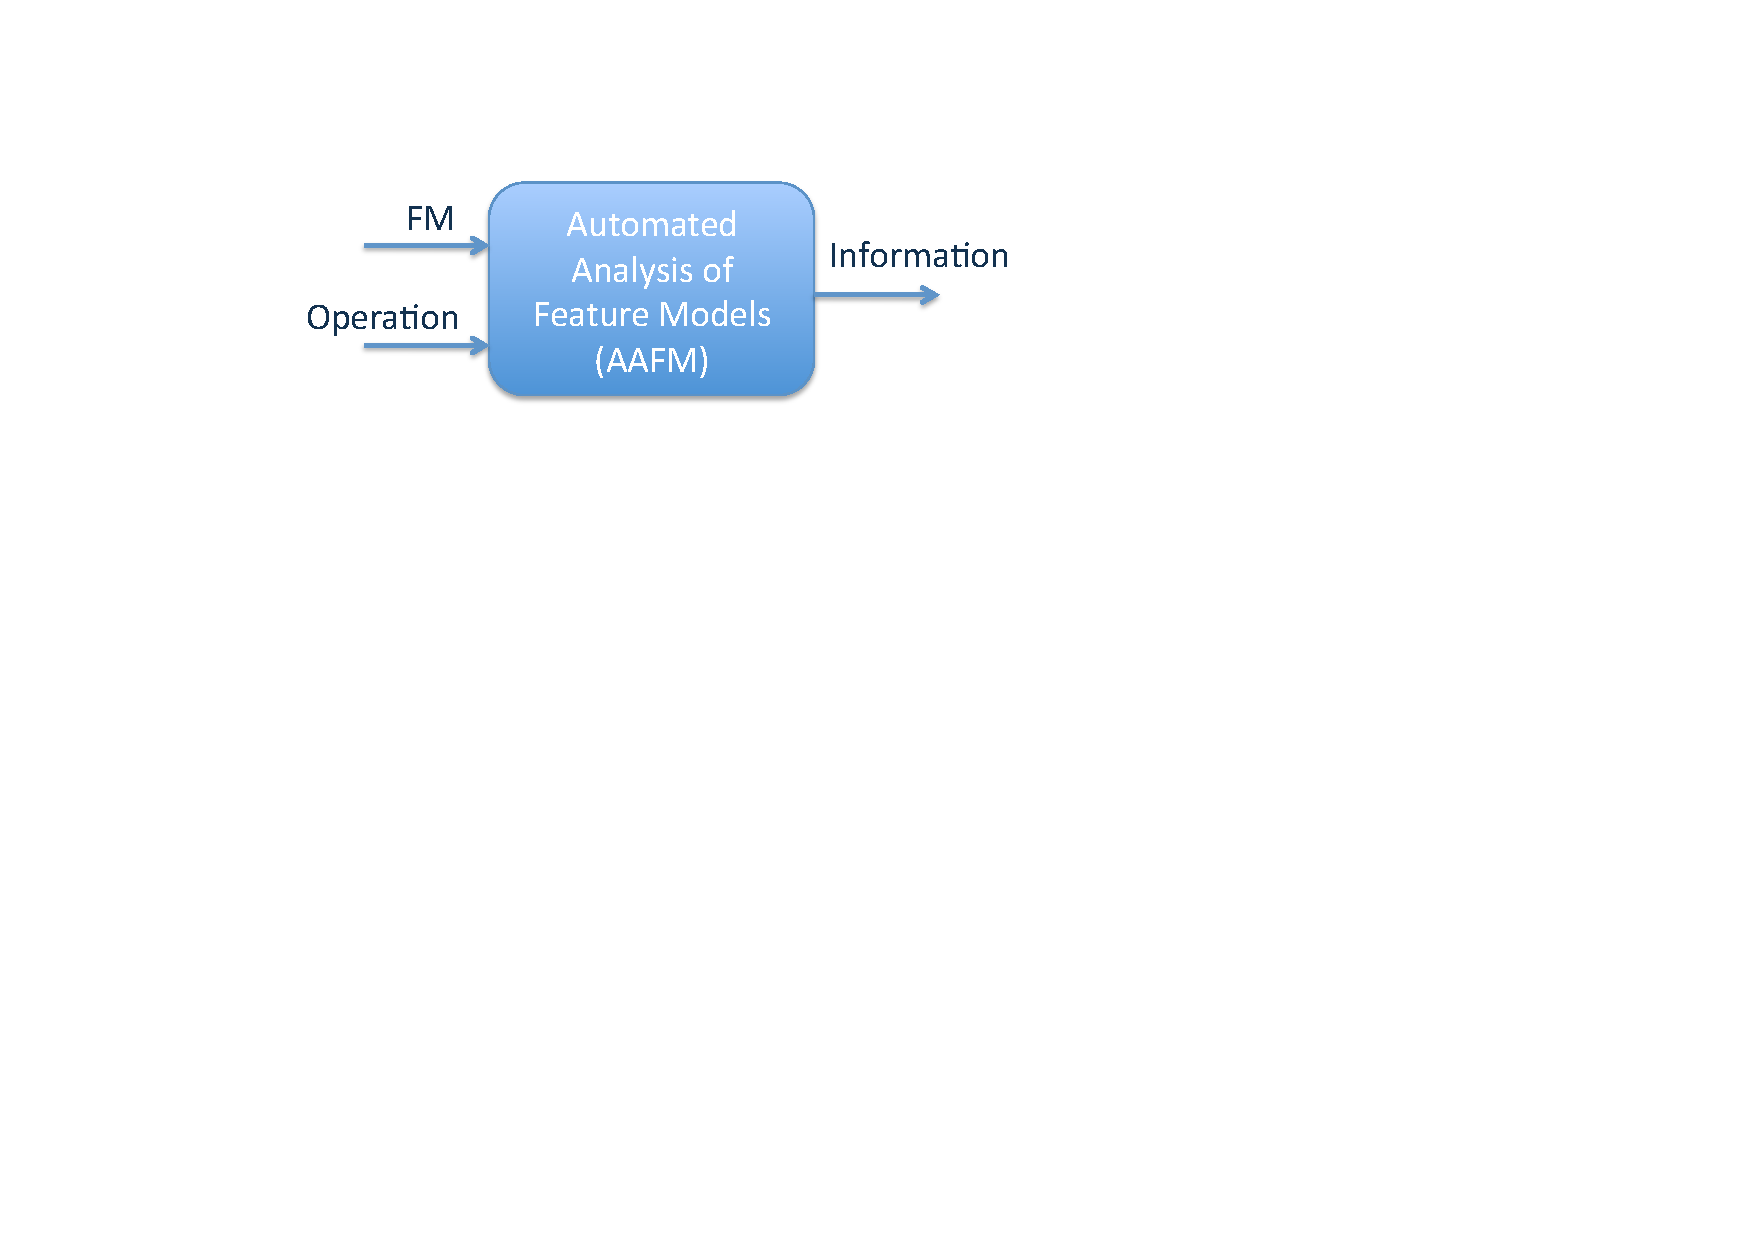
\includegraphics[width=0.30\textwidth]{figures/introduction/oldAAFM.pdf}
		\label{fig:oldBlackBox}
	}
		\subfigure[Extending the AAFM process with explanations]{
		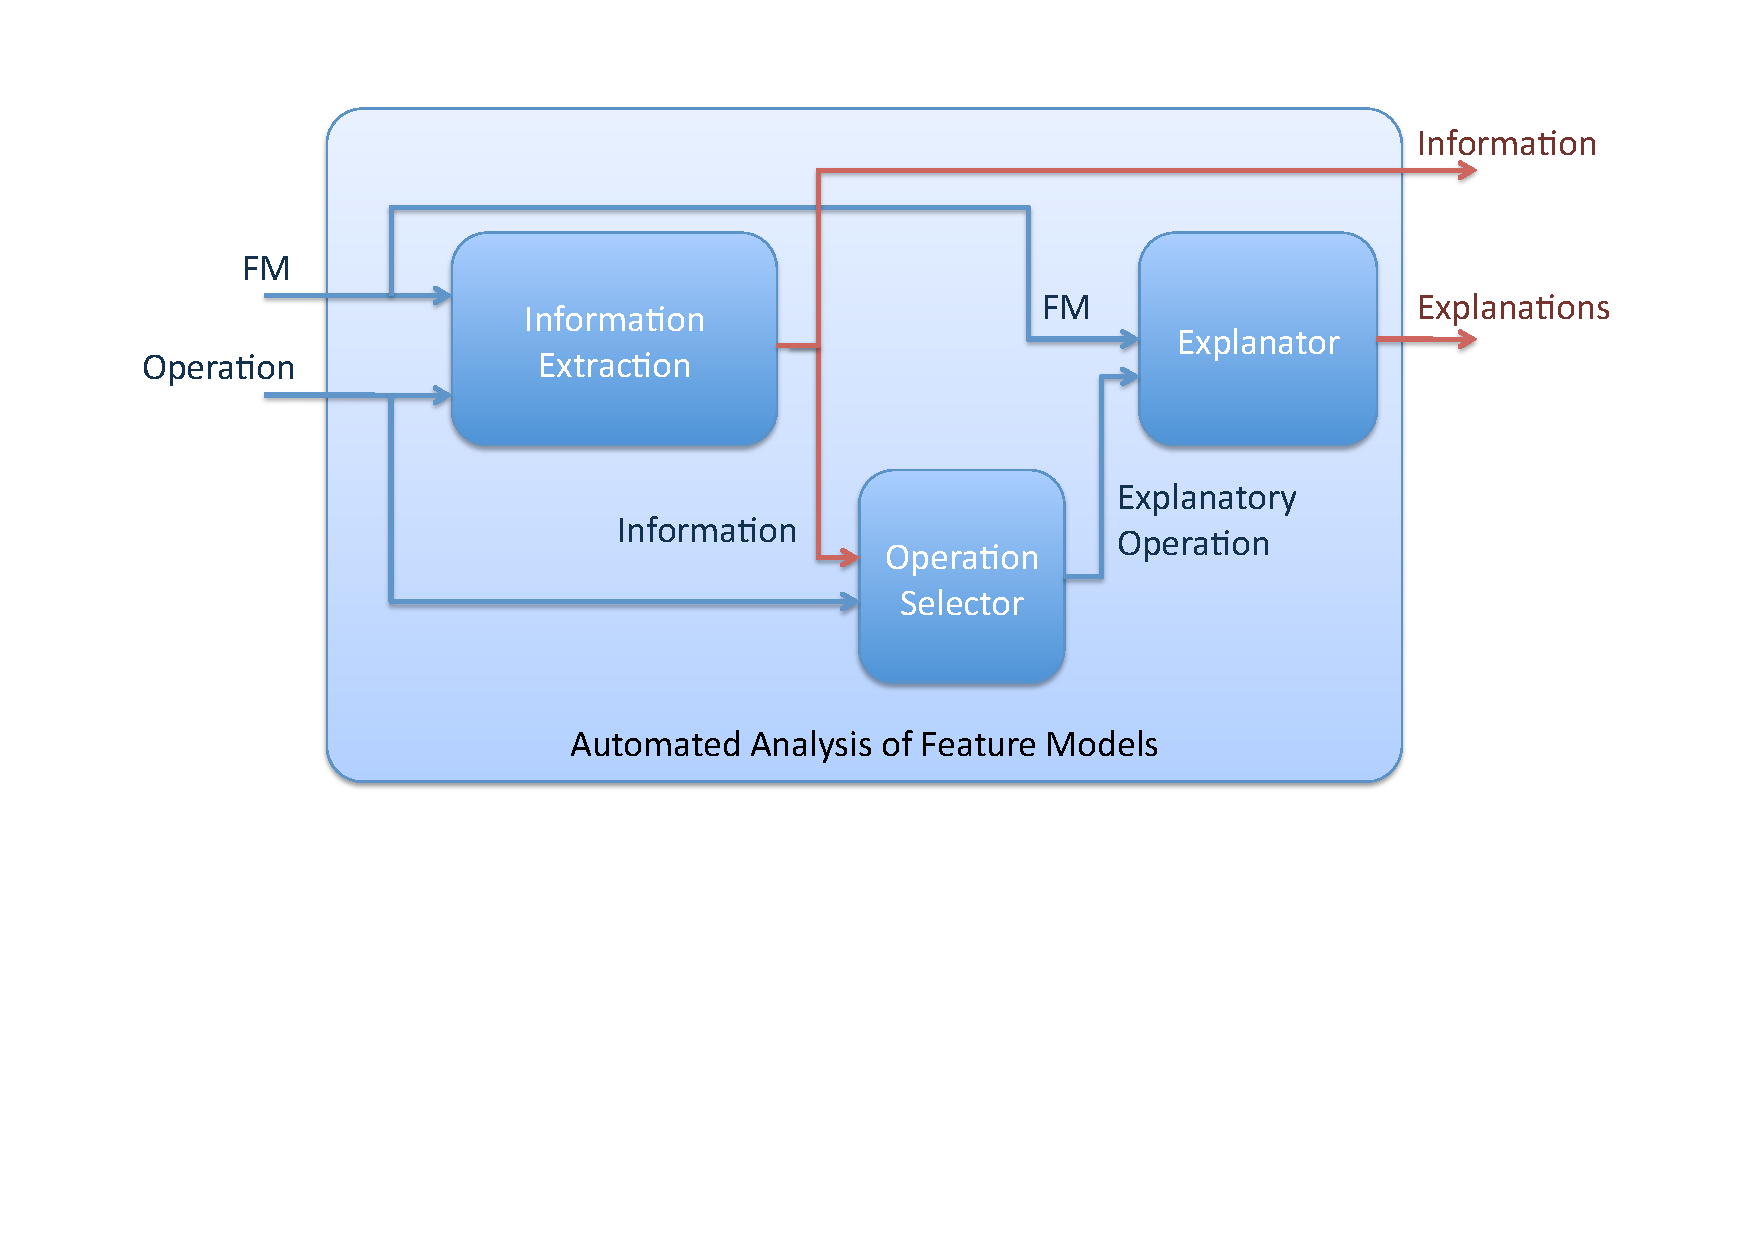
\includegraphics[width=0.65\textwidth]{figures/introduction/newAAFM.pdf}
		\label{fig:newBlackBox}
	}
		%\missingfigure{Several architectures and a structural model for each of them (Slide 3)}
		
	\caption{A different view on AAFM distinguishing between information extraction and explanatory operations}
	\label{fig:AAFM}
\end{figure}

However, there is a subset of analysis operations known as \emph{explanatory operations} (EO) whose objective is explaining the result obtained from a IEO. Sometimes, the result is not the expected one and the analyser needs to know which are the relationships that have caused it. For example, let us suppose that the IEO 'which are the products described in a FM that cost less than \$1000?' obtains no products as a result. If we were expecting to obtain at least one product, it is important to determine the relationships in the FM that are responsible of that behaviour, so an EO 'why there is no product costing less than \$1000?' will shed light on the relationships that avoid obtaining any product. Obtaining no result is not the only case that claims for explanations. If we obtained only one product as a result and we were expecting to obtain at least 10 products, although an answer is obtained the result is unexpected and the discrepancy reasons have to be found. Moreover, explanatory operations are also useful even when an expected result is obtained, to reinforce the certainty that the result is correct. So it can be concluded that EOs complement the information an FM analyser obtains from IEOs.

The complexity of feature modelling relies on correctly setting the relationships that describe the set of products to be built in a SPL. Relationships are the only elements responsible of the results obtained in FM analysis. So an \emph{explanation} is a set of relationships that may have caused that result. While IEO provides for an unique response that is known for certain, an EO provides for a set of probable explanations to a result obtained from a IEO, being only one of them a valid explanation. It would be the analyser the one in charge of discriminating the correct explanation, maybe performing new analysis operations.

\sidetext{This is a side text. Use to remark important information}

Therefore, two kinds of operations are distinguished in AAFM: information extraction and explanatory operations. Explanatory operations have no sense without a paired information extraction operation and its result. To ensure that explanatory operations are always paired to an information extraction operation, we define a new black-box process of AAFM that incorporates explanations as an additional output (see Figure \ref{fig:newBlackBox})

\begin{enumerate}
\item Information extraction: the original process, which remains the same.
\item Operation selector: depending on the information extraction operation the analyser asks for and the information obtained as a result, this process provides the explanatory operation to be performed. In other words, it pairs an explanatory operation to an information extraction operation.
\item Explanatory analysis: provides a set of explanations from the FM and the explanatory operation.
\end{enumerate} 

The overall process can be encapsulated into a holistic black-box process which receives the FM and the information extraction operation as inputs and provides a result and explanations as outputs. It can be seen as we just add explanations as an output to the analysis process. 

To realise this view on the AAFM, we need to give details on the insides of these black-boxes. Since the information extraction process is already rigourously defined in Benavides' PhD dissertation, the purpose of this paper is defining the remaining two sub-processes. We formalise the explanatory analysis process by means of default logic and provide the criteria to implement the operation selector process.

Most Common Techniques to perform AAFM Operations.


\section{Dynamic Software Product Lines (DSPL)}
What is a \dspl. Different points of view. What is important is the automation of reconfiguration properties relying on \spl techniques.

We focus in the application of explanations in \dspls as an application of our results. Specifically we have worked in MAS and smart homes providing a solution for automating product reconfiguration.

\section{Hypothesis and Objectives}

\objective{Justifying that explanations are a particular set of operations in AAFM that are not solvable by means of the techniques that are used up-to-date}
\objective{Set an impacting phrase that summarises the hypothesis}
\importantframe{Hypothesis}{Explanations cannot be solved by AI techniques used to solve AAFM. There should exist other AI techniques to solve explanations. }

\importantframe{Objective of the dissertation}{Defining a framework to provide solutions for explanatory analysis in FMs.}

This dissertation summarises our contribution to solve some of the objectives we set in our PhD project. 

\begin{itemize}
\item Defining a catalog of analysis operations where explanations are applied.
\item Rigorously defining these operations in terms of logics.
\item Proposing solutions to these operations.
\item Validating our results by means of tools and projects where they are applied. 
\end{itemize}

Next chapter focuses on refining how we have contributed to deal with the above objectives.

A piece of code...

\begin{lstlisting}[style=javacode]
public Map<Cardinality,CardinalValue> detectWrongCardinals() {
	// any other implementation of Map can be used instead.
	Map<Cardinality,CardinalValue> result = 
		new TreeMap<Cardinality,CardinalValue>();
	for( r : relationships) {
		if (r instanceof Set) {
			Set set = (Set)r;
			Cardinality card = set.getCardinality();
			Domain dom = card.getDomain();
			for (value: dom.getValues())
				if (isWrongCardinal(card,value))
					result.put(card,value);
		}
	}
	return result;
}
\end{lstlisting}

A coolTable. Use inside a table.
\begin{table*}[h!]
	\centering
	\begin{coolTable}{lcc}{3} % 3 is the only addition to standard tabular environment
	% lcc is the alignment for each columns. 3 is the total number of columns of the table.
{A Catalog of FM Explanatory Operations (2009 version)}
			\textbf{Information Extraction Operation}&\multicolumn{2}{c}{\textbf{FM Explanatory Operations}}\\
			\midrule
			% Always use midrules instead of \hline. It adds an extra vertical space that helps to improve the clarity
			&\textit{Why? operation}&\textit{Why not? operation}\\
			\cmidrule(r){2-3} % use cmidrule instead of \cline.
			Valid FM&-&invalid FM \\
			Valid Configuration&valid partial conf.&invalid partial conf.\\		
			Valid Product&valid product&invalid product\\
			Products Listing&vaild Product/Config&invalid FM/Product/Config\\
			Products Counting&vaild Product/Config&invalid FM/Product/Config\\
			Optimisation&vaild Product/Config&invalid FM/Product/Config\\
			Core feature&core feature&core feature\\
			Variant feature&variant feature&variant feature\\
			Dead feature detection&-&dead feature\\
			False-optional feature detection&-&false-optional feature\\
			Wrong-cardinality detection&-&wrong cardinal\\
			%\multirow{2}{*}{\textbf{Information Extraction Operation}}
			\textbf{Information Extraction Operation}&\multicolumn{2}{c}{\textbf{Configuration Explanatory Operations}}\\
			\midrule
			&\textit{Why? operation}&\textit{Why not? operation}\\
			\cmidrule(r){2-3}
			Valid Configuration&valid partial conf.&invalid partial conf.\\	
		\end{coolTable}
	\caption{Most frequently used explanatory operations and their corresponding information extraction operations}
	\label{tab:listDeductiveAbductive}
\end{table*}

Use \textbackslash TableSubtitle\{n,title\} to add a subtitle as the header. n is the number of columns and title is the text to place. \citep{benavides05-CAISE}

\lineNumbersOff

%\glossarystyle{long}
\printglossaries
\newpage

\bibliographystyle{abbrvnat}
\addcontentsline{toc}{chapter}{Referencias bibliográficas}
\bibliography{referencias}

\end{document} 